\documentclass[11pt]{article}

% --- Paquetes de configuración ---
\usepackage{ifxetex}
\ifxetex
  \usepackage{fontspec}
\else
  \usepackage[utf8]{inputenc}
  \usepackage[T1]{fontenc}
\fi
\usepackage[spanish,es-tabla]{babel}

% --- Geometría de página ---
\usepackage[top=1.65cm, bottom=1.65cm, left=2.2cm, right=2.2cm]{geometry}

% --- Matemáticas y tablas ---
\usepackage{amsmath, amssymb}
\usepackage{booktabs}
\usepackage{xltabular}
\usepackage{array}
\usepackage{enumitem}
\usepackage{graphicx}
\usepackage{xcolor}

% --- Enlaces ---
\usepackage[colorlinks=true, linkcolor=blue!80!black, citecolor=blue!80!black, urlcolor=blue!80!black]{hyperref}

% --- Configuración de párrafos e interlineado ---
\setlength{\parskip}{0.18em}
\setlength{\parindent}{0pt}
\setlist{nosep, leftmargin=1.35em, itemsep=0.12em}

\begin{document}

% --- Encabezado idéntico al formato original ---
\begin{center}
    {\Large \textbf{Comprensión del Contexto, Análisis Visual y Caracterización de Brechas Globales de Bienestar}}\\[0.3em]
    {\large \textbf{World Happiness Report 2024}}\\[0.4em]
    {\normalsize Proyecto 2 --- Visualización Reproducible en Python}\\[0.6em]
    Arnold Santiago Torres Anzola\\
    Juan David Cruz Romero
\end{center}

\vspace{0.2em}

% ==============================================================================
% 1. COMPRENSIÓN DEL CONTEXTO
% ==============================================================================
\section{Comprensión del Contexto}

El \textit{World Happiness Report 2024} (WHR 2024) analiza el bienestar subjetivo a nivel global a partir de las evaluaciones de vida recopiladas mediante la Encuesta Mundial de Gallup (\textit{Gallup World Poll}). Dicha medición emplea la escalera de Cantril (\textit{Cantril Self-Anchoring Striving Scale}), un instrumento psicométrico en el que los encuestados evalúan su vida actual en una escala de 0 a 10, donde el peldaño 0 representa la peor vida posible y el 10 la mejor vida alcanzable (reportada como promedio móvil trienal nacional para el periodo 2021--2023, consolidando 143 países).

Para explicar las diferencias observadas entre naciones, el informe utiliza un modelo econométrico de descomposición aditiva basado en una referencia estandarizada denominada \textit{Distopía} (un país ficticio cuyos indicadores corresponden a los mínimos históricos observados internacionalmente, con un puntaje base de evaluación $\approx 1.97$ puntos), sumada a la contribución en puntos de seis factores explicativos clave: PIB per cápita, apoyo social, esperanza de vida saludable, libertad de elección vital, generosidad y percepción de corrupción, junto al residuo econométrico no modelado (\textit{Dystopia + residual}).

En cumplimiento de las directrices del proyecto, el marco analítico se restringe exclusivamente al archivo oficial mandatorio \texttt{WHR24\_Data\_Figure\_2.1.xls} (143 observaciones nacionales y 11 variables), asumiendo el rol de científicos de datos responsables de estructurar una exploración reproducible orientada a examinar los patrones de relación entre dichos indicadores y la calidad de vida de las poblaciones.

% ==============================================================================
% 2. AUDIENCIA TÉCNICA
% ==============================================================================
\section{Audiencia Técnica Específica}

La audiencia técnica está delimitada concretamente al \textbf{Equipo Técnico de Análisis Comparativo de Bienestar y Políticas Públicas de un Organismo Multilateral de Desarrollo} (homólogo a la Unidad de Estadísticas y Bienestar Social del PNUD o la Dirección de Estadísticas de la OCDE).

Este equipo especializado está integrado por economistas aplicados, analistas cuantitativos y científicos de datos que evalúan diagnósticos comparativos internacionales sobre las condiciones de vida entre naciones. Su interés técnico concreto radica en comprender cómo interactúan las variables de orden material (PIB per cápita y salud) con las dimensiones cívico-sociales e institucionales (apoyo social, libertad y probidad pública) al caracterizar las brechas de bienestar, contrastando perfiles de países y evaluando en qué medida factores sociales amortiguan o potencian el bienestar. Para ello, requieren un flujo de trabajo reproducible, trazabilidad metodológica completa y rigurosa \textit{cautela inferencial}, evitando atribuir causalidad a datos de naturaleza puramente observacional y transversal.

% ==============================================================================
% 3. PREGUNTA ANALÍTICA
% ==============================================================================
\section{Pregunta Analítica Central y Subpreguntas}

Para responder a las demandas del equipo técnico multilateral sin incurrir en aseveraciones causales indebidas, se formula la siguiente pregunta central de investigación:

\begin{quote}
\textit{«¿Qué variables se asocian con la calidad de vida y evaluación del bienestar de los países, qué diferencias se evidencian entre naciones y de qué manera las condiciones económicas, de salud y socioinstitucionales diferencian a los países con alta y baja evaluación vital en el World Happiness Report 2024?»}
\end{quote}

\textbf{Subpreguntas y objetivos operativos:}
\begin{enumerate}
    \item \textbf{Diferenciación Empírica Cuartílica:} ¿En qué componentes específicos (económico, de salud y socioinstitucional) se concentran las mayores brechas absolutas y estandarizadas entre el 25\% superior ($Q4$) y el 25\% inferior ($Q1$)?
    \item \textbf{Capacidad Explicativa Relativa:} ¿En qué medida el ingreso por habitante (PIB per cápita) es suficiente por sí solo para explicar los niveles de bienestar, o qué papel amortiguador desempeñan las redes de apoyo social y la confianza institucional?
    \item \textbf{Casos Atípicos y Resiliencia Comunitaria:} ¿Qué naciones logran evaluaciones de vida significativamente superiores o inferiores a lo predicho por su nivel de ingreso, y qué factores explican dicha divergencia?
\end{enumerate}

% ==============================================================================
% 4. VARIABLES EN EL WORLD HAPPINESS REPORT 2024
% ==============================================================================
\section{Variables en el World Happiness Report 2024}

\textit{Diccionario y Documentación de Variables para Análisis y Visualización}

\vspace{0.4em}

\begin{xltabular}{\textwidth}{>{\bfseries\raggedright\arraybackslash}p{2.8cm} >{\raggedright\arraybackslash}p{3.5cm} >{\raggedright\arraybackslash}p{3.5cm} >{\raggedright\arraybackslash}X}
\caption{Diccionario y especificación de variables del World Happiness Report 2024.} \label{tab:variables_whr2024} \\
\toprule
Variable & ¿Qué es? & ¿Cómo se mide? & ¿Qué significa / Interpretación? \\
\midrule
\endfirsthead

\multicolumn{4}{c}%
{{\bfseries \tablename\ \thetable{} -- Continuación de la página anterior}} \\
\toprule
Variable & ¿Qué es? & ¿Cómo se mide? & ¿Qué significa / Interpretación? \\
\midrule
\endhead

\midrule
\multicolumn{4}{r}{{Continúa en la siguiente página...}} \\
\bottomrule
\endfoot

\bottomrule
\endlastfoot

Country name & Identificador geográfico territorial. & Cadena de texto con el nombre oficial del país (143 registros). & Unidad básica de observación y desagregación analítica internacional. \\
\addlinespace[3pt]
Ladder score & Variable objetivo (dependiente). Evaluación global de calidad de vida. & Encuesta Gallup World Poll. Escala de 0 a 10 (0 = peor vida, 10 = mejor vida). Promedio móvil trienal. & Refleja el nivel general de satisfacción y bienestar subjetivo reportado por la población. Métrica central del reporte. \\
\addlinespace[3pt]
upperwhisker / lowerwhisker & Intervalo de confianza de la evaluación de vida. & Escala de 0 a 10. Límites superior e inferior estimados al 95\% de confianza. & Expresa la precisión estadística y variabilidad muestral del \textit{Ladder score} en cada país. \\
\addlinespace[3pt]
Explained by: Log GDP per capita & Contribución de la prosperidad económica por habitante. & Puntos de la escala explicados por $\ln(\text{PIB PPA})$ (Banco Mundial / WDI). & Dimensión económica. Expresa los rendimientos marginales decrecientes del ingreso sobre la calidad de vida. \\
\addlinespace[3pt]
Explained by: Social support & Contribución de las redes de auxilio y apoyo social. & Proporción nacional que responde «sí» a contar con amigos o familiares en momentos difíciles. & Refleja la solidez del tejido social y el respaldo comunitario ante situaciones de vulnerabilidad o crisis. \\
\addlinespace[3pt]
Explained by: Healthy life expectancy & Contribución de la salud física y longevidad funcional. & Estimaciones OMS: promedio de años esperados de vida en buen estado de salud funcional al nacer. & Evalúa la dimensión fisiológica y el impacto de la ausencia de enfermedades o discapacidades limitantes. \\
\addlinespace[3pt]
Explained by: Freedom to make life choices & Contribución de la autonomía y libertad vital. & Proporción de la población satisfecha con su libertad para elegir qué hacer con su vida (0 a 1). & Medida de autodeterminación y oportunidades de realización personal percibidas sin coacciones. \\
\addlinespace[3pt]
Explained by: Generosity & Contribución del comportamiento prosocial y solidario. & Residuo de donaciones benéficas monetarias en el último mes, controlado por el PIB per cápita. & Captura la disposición solidaria y altruista de la sociedad con independencia de su capacidad adquisitiva. \\
\addlinespace[3pt]
Explained by: Perceptions of corruption & Contribución de la confianza institucional y gobernanza. & Promedio de percepción sobre extensión de corrupción en entidades del gobierno y empresas (0 a 1). & Mide la integridad institucional. Mayores contribuciones indican menor corrupción percibida en el entorno. \\
\addlinespace[3pt]
Dystopia + residual & Línea base de Distopía más residuo no modelado. & Puntaje base de Distopía ($\approx 1.97$) más el residuo econométrico no capturado por los 6 factores. & Garantiza la descomposición aditiva y cuantifica la proporción del bienestar debida a factores no medidos. \\
\end{xltabular}

\vspace{0.6em}

% ==============================================================================
% 5. INTERPRETACIÓN ESCRITA DE LAS VISUALIZACIONES (NUMERAL 8)
% ==============================================================================
\section{Interpretación Analítica de las Visualizaciones (Numeral 8)}

En concordancia con el flujo del proyecto, una vez importados, inspeccionados y limpiados los datos en el cuaderno reproducible de Python (\texttt{notebooks/EquipoX\_Proyecto2\_Visualizacion.ipynb}), se procedió a la construcción de las visualizaciones estáticas e interactivas planificadas. A continuación se presentan las interpretaciones escritas inmediatas de cada visualización, vinculadas directamente con la pregunta analítica formulada.

\subsection{Criterio de Segmentación Cuartílica y Preparación Comparativa}
Para contrastar empíricamente a los países con mayor y menor evaluación vital de forma reproducible y estadísticamente balanceada, se adoptó el criterio de segmentación por cuartiles del 25\% sobre el \textit{Ladder score} ($N = 143$):
\begin{itemize}
    \item \textbf{Cuartil Superior ($Q4$ - Alto Bienestar):} 36 naciones con puntajes $\ge 6.416$ puntos (desde Finlandia con 7.741 hasta España con 6.421 pts; media del grupo = 6.88 pts; desv. est. = 0.35 pts).
    \item \textbf{Cuartil Inferior ($Q1$ - Bajo Bienestar):} 36 naciones con puntajes $\le 4.726$ puntos (desde Pakistán con 4.657 hasta Afganistán con 1.721 pts; media del grupo = 3.91 pts; desv. est. = 0.62 pts).
    \item \textbf{Segmento Central Intermedio ($Q2-Q3$):} 71 naciones con evaluaciones intermedias (mediana global = 5.79 pts; media global = 5.53 pts).
\end{itemize}

\textbf{Tratamiento de casos especiales:} Baréin, Tayikistán y Estado de Palestina poseen \textit{Ladder score} pero carecen de contribuciones explicativas, por lo que se incluyeron en la clasificación global pero se excluyeron de los análisis multidimensionales ($n = 140$). Venezuela registra $\text{PIB} = 0.000$ (se excluyó de los ajustes lineales sobre el ingreso) y Líbano presenta un residuo negativo en \textit{Distopía + residuo} ($-0.073$ pts), reflejo de un colapso estructural severo.

\subsection{Matriz Comparativa de Brechas ($Q4 - Q1$)}
La Tabla~\ref{tab:brechas_analisis} sintetiza las contribuciones promedio en puntos de la escala de Cantril por cuartil, la brecha absoluta, la brecha estandarizada (dividida por la desviación estándar combinada de ambos grupos) y la existencia de traslape empírico entre observaciones extremas.

\begin{table}[h!]
\centering
\small
\renewcommand{\arraystretch}{1.05}
\caption{Matriz comparativa de contribuciones promedio por cuartil y descomposición de la brecha $Q4 - Q1$.}
\label{tab:brechas_analisis}
\vspace{0.3em}
\begin{tabularx}{\textwidth}{>{\raggedright\arraybackslash}p{4.0cm} cccc >{\raggedright\arraybackslash}X}
\toprule
\textbf{Componente / Dimensión Analítica} & \textbf{Q1 (pts)} & \textbf{Q4 (pts)} & \textbf{Brecha (pts)} & \textbf{Brecha ($z$)} & \textbf{¿Traslape $Q1-Q4$?} \\
\midrule
PIB per cápita (Dimensión Económica) & 0.92 & 1.82 & \textbf{+0.90} & 3.9 desv. est. & Sí ($[0.53, 1.45]$ vs $[1.27, 2.14]$) \\
Apoyo social (Dimensión Socioinstitucional) & 0.74 & 1.41 & \textbf{+0.67} & 3.1 desv. est. & Sí ($[0.00, 1.28]$ vs $[1.08, 1.62]$) \\
Esperanza de vida saludable (Dimensión Salud) & 0.35 & 0.66 & \textbf{+0.32} & 3.2 desv. est. & Sí ($[0.00, 0.59]$ vs $[0.51, 0.77]$) \\
Libertad para decidir (Socioinstitucional) & 0.49 & 0.74 & \textbf{+0.25} & 1.8 desv. est. & Sí ($[0.00, 0.86]$ vs $[0.53, 0.86]$) \\
Probidad pública / Percepción de corrupción & 0.12 & 0.29 & \textbf{+0.17} & 1.5 desv. est. & Sí ($[0.01, 0.26]$ vs $[0.01, 0.57]$) \\
\midrule
\textbf{Suma Socioinstitucional (3 comp.)} & \textbf{1.35} & \textbf{2.44} & \textbf{+1.09} & \textbf{3.5 desv. est.} & \textbf{No (Casi nulo: $1.953$ vs $1.959$)} \\
Generosidad (Comportamiento prosocial) & 0.15 & 0.17 & +0.02 & 0.2 desv. est. & Sí (Prácticamente no discrimina) \\
Distopía + residuo (Componente no modelado) & 1.15 & 1.79 & +0.65 & 1.3 desv. est. & Sí (Peso relevante: 22.0\% de la brecha) \\
\midrule
\textbf{Evaluación Global de Vida (Ladder score)} & \textbf{3.91} & \textbf{6.88} & \textbf{+2.96} & \textbf{4.2 desv. est.} & \textbf{No (Segmentación por definición)} \\
\bottomrule
\end{tabularx}
\end{table}

\begin{figure}[h!]
\centering
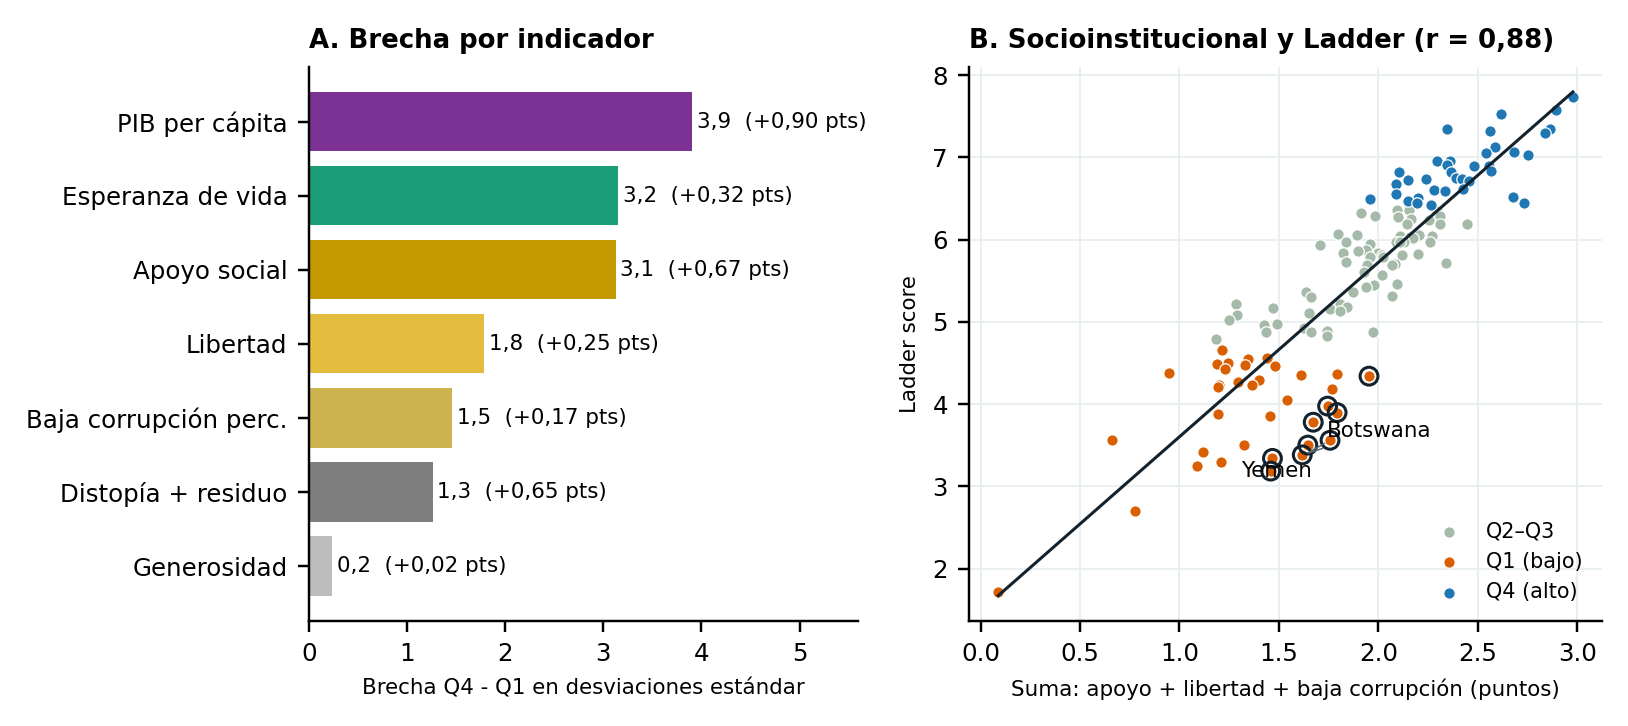
\includegraphics[width=0.76\textwidth]{figura_resumen_brechas.png}
\caption{\textbf{(A)} Brecha estandarizada $Q4 - Q1$ por indicador (entre paréntesis, diferencia en puntos). \textbf{(B)} Relación econométrica MCO entre la Dimensión Socioinstitucional y el Ladder score ($r=0.88, n=140$), con identificación de países atípicos.}
\label{fig:graficos_resumen}
\end{figure}

\subsection{Interpretación Detallada de las Visualizaciones del Proyecto}

\subsubsection{Figura 1 (Seaborn): Distribución Empírica del Bienestar y Puntos de Corte Cuartílicos}
\begin{itemize}
    \item \textbf{Qué necesita examinar el analista:} La forma general de la distribución del \textit{Ladder score} a nivel global, evaluando si el bienestar se distribuye normalmente o si existen sesgos sistemáticos que justifiquen el análisis segmentado.
    \item \textbf{Patrón observado:} La distribución muestra una concentración predominante en valores intermedios (mediana global = 5.79 pts; media = 5.53 pts). La mediana supera a la media, revelando una marcada asimetría negativa (cola hacia la izquierda): naciones con evaluaciones extremadamente deterioradas, como Afganistán (1.72 pts), arrastran el promedio general hacia abajo, contrastando con el techo alcanzado por Finlandia (7.74 pts).
    \item \textbf{Aporte a la pregunta analítica:} Justifica plenamente la comparación de los cuartiles extremos $Q1$ y $Q4$ como grupos contrastantes no redundantes, cuya distancia entre medianas es de 2.70 puntos (y 2.96 puntos entre medias).
    \item \textbf{Cautela inferencial:} El histograma documenta la dispersión psicométrica de la variable dependiente, pero no explica los factores determinantes de dicha disparidad.
\end{itemize}

\subsubsection{Figura 2 (Seaborn): Descomposición de la Brecha Absoluta y Estandarizada por Componente}
\begin{itemize}
    \item \textbf{Qué necesita examinar el analista:} En qué factores específicos del modelo de regresión se originan las mayores distancias entre las naciones más prósperas y las más vulnerables.
    \item \textbf{Patrón observado:} El PIB per cápita registra la mayor brecha individual (+0.90 puntos de la escala), seguido de cerca por el apoyo social (+0.67 pts), la esperanza de vida saludable (+0.32 pts), la libertad vital (+0.25 pts) y la probidad pública (+0.17 pts). La generosidad (+0.02 pts) prácticamente no discrimina entre grupos.
    \item \textbf{Análisis estandarizado:} Al normalizar por la dispersión conjunta (desviaciones estándar), el PIB (3.9 $z$), la salud (3.2 $z$) y el apoyo social (3.1 $z$) exhiben una capacidad de separación prácticamente empatada, confirmando que la brecha global no es un fenómeno puramente monetario.
    \item \textbf{Cautela inferencial:} Los puntos de la escalera dependen de los coeficientes de regresión del informe oficial del WHR; no representan magnitudes causales autónomas.
\end{itemize}

\subsubsection{Figura 3 (Seaborn): Anatomía Aditiva de los Puntajes Promedio de $Q1$ y $Q4$}
\begin{itemize}
    \item \textbf{Qué necesita examinar el analista:} Cuál es la estructura interna de los puntajes agregados en ambos grupos y qué proporción de la brecha total de +2.96 puntos corresponde a cada componente.
    \item \textbf{Patrón observado:} En ambos cuartiles, los tramos principales del puntaje son el PIB per cápita, el apoyo social y \textit{Distopía + residuo}. Del total de la brecha de 2.96 puntos: el PIB explica el 30.4\%, el conjunto socioinstitucional explica el 36.8\%, la salud física el 10.8\%, la generosidad menos del 1.0\%, y \textit{Distopía + residuo} explica un notable 22.0\% (+0.65 pts).
    \item \textbf{Aporte a la pregunta analítica:} Demuestra que las condiciones socioinstitucionales superan al ingreso material en su peso acumulado sobre la desigualdad de bienestar global, y que más de una quinta parte de la brecha responde a factores no modelados (crisis humanitarias y particularidades culturales).
\end{itemize}

\subsubsection{Figura 4 (Seaborn): Contribución Económica (PIB) y Detección de Países Atípicos}
\begin{itemize}
    \item \textbf{Qué necesita examinar el analista:} La fortaleza de la relación bivariada entre el ingreso y el bienestar, y la identificación de naciones que exhiben rendimientos significativamente desacoplados de su prosperidad económica.
    \item \textbf{Patrón observado:} Existe una relación positiva robusta ($r = 0.80, R^2 = 0.64, n = 139$ excluyendo a Venezuela), pero con una dispersión residual de 36\% que el ingreso por sí solo no acompaña.
    \item \textbf{Países por encima de la recta (sobre-rendimiento y resiliencia):} Nicaragua (+1.43 pts de residuo), Mozambique (+1.61 pts) y El Salvador (+1.22 pts), cuyas poblaciones alcanzan niveles de bienestar comparables a economías de mayor ingreso gracias a la densidad de sus redes de apoyo social y capital comunitario.
    \item \textbf{Países por debajo de la recta (vulnerabilidad y colapso):} Líbano ($-2.80$ pts), Botsuana ($-2.28$ pts) y Afganistán ($-2.05$ pts). En estos países, el intervalo de confianza al 95\% del \textit{Ladder score} no incluye la recta de regresión, demostrando que su rezago no obedece a error muestral sino a severos déficits institucionales y fracturas del entorno cívico.
\end{itemize}

\subsubsection{Figura 5 (Plotly Interactivo): Dimensión Socioinstitucional y Separación sin Traslape}
\begin{itemize}
    \item \textbf{Qué necesita examinar el analista:} Si la articulación conjunta de las variables de convivencia cívica e institucional (apoyo social + libertad + probidad) genera un ordenamiento más potente que el ingreso económico.
    \item \textbf{Patrón observado:} La correlación entre la dimensión socioinstitucional y el \textit{Ladder score} es de $r = 0.88 (n = 140)$, superando ampliamente a la correlación económica ($r = 0.77$ para las mismas 140 naciones). Más relevante aún: mientras en los indicadores individuales siempre hay solapamiento entre naciones de $Q1$ y $Q4$, en la suma socioinstitucional la separación es casi perfecta: el país con mayor puntaje en $Q1$ llega a 1.953 (Camboya) y el menor en $Q4$ inicia en 1.959 (Rumania).
    \item \textbf{Valor de la interactividad:} Permite al investigador pasar el cursor para leer el vector completo de factores por país, aislar cuartiles y profundizar en las naciones frontera.
    \item \textbf{Cautela inferencial:} Al sumar tres variables, el rango matemático de la dimensión se amplía; además, como los componentes suman el puntaje, parte de la correlación es mecánica y descriptiva.
\end{itemize}

\subsubsection{Figura 6 (Plotly Interactivo): Heterogeneidad Intra-Grupo País por País}
\begin{itemize}
    \item \textbf{Qué necesita examinar el analista:} Si los países pertenecientes al mismo cuartil comparten una estructura homogénea o si existen divergencias críticas internas.
    \item \textbf{Patrón observado:} El cuartil superior ($Q4$) es sumamente cohesionado (desv. est. de 0.35 pts), con aportes elevados y consistentes en PIB y apoyo social en todas las naciones. Por el contrario, el cuartil inferior ($Q1$) es profundamente heterogéneo (desv. est. de 0.62 pts): Afganistán exhibe contribución de 0.00 en apoyo social y libertad, mientras que naciones como Chad registran aportes de apoyo social sustantivos pero combinados con un colapso en otras áreas. Asimismo, el residuo no explicado en $Q1$ fluctúa desde $-0.07$ (Líbano) hasta $+2.12$ (Chad).
    \item \textbf{Valor de la interactividad:} El menú selector permite alternar de inmediato entre cuartiles y desactivar componentes en la leyenda para comparar únicamente las contribuciones explicadas.
\end{itemize}

% ==============================================================================
% 6. SÍNTESIS DE HALLAZGOS Y RESPUESTA A LA PREGUNTA (NUMERAL 9)
% ==============================================================================
\section{Síntesis de Hallazgos y Respuesta a la Pregunta Analítica (Numeral 9)}

A partir de la evidencia cuantitativa, tabular y gráfica consolidada en el estudio, se sintetizan las siguientes respuestas directas a la pregunta central de investigación formulada para el equipo técnico multilateral:

\begin{enumerate}[leftmargin=1.5em, itemsep=0.35em]
    \item \textbf{El ingreso económico es condición necesaria pero no suficiente (+0.90 pts):} El PIB per cápita explica la mayor brecha individual entre los cuartiles extremos (30.4\% de la distancia total). La base material y la productividad protegen a las sociedades contra la indigencia y permiten el financiamiento de infraestructura básica; no obstante, un enfoque centrado exclusivamente en el crecimiento económico generará diagnósticos incompletos, dado que la economía por sí sola deja un 36\% de varianza sin explicar.
    \item \textbf{La condición socioinstitucional constituye el principal divisor del bienestar humano (+1.09 pts):} La concurrencia de apoyo social (+0.67 pts), libertad de elección vital (+0.25 pts) y probidad pública (+0.17 pts) representa el 36.8\% del diferencial global de bienestar. La fortaleza de estas redes comunitarias es lo que explica que economías emergentes alcancen evaluaciones vitales equiparables a las de Europa Occidental, mientras que su ausencia o deterioro precipita a naciones de ingreso medio a los puestos más bajos de la escala mundial.
    \item \textbf{La salud física actúa como pilar funcional intermedio (+0.32 pts):} La longevidad saludable genera una separación neta de 3.2 desviaciones estándar, consolidándose como un requisito indispensable de funcionalidad y calidad de vida.
    \item \textbf{Solidaridad prosocial no discriminante (+0.02 pts):} Las conductas de generosidad y donaciones monetarias ocurren con similar intensidad en naciones ricas y pobres, careciendo de capacidad predictiva para explicar las brechas estructurales de desarrollo.
    \item \textbf{Magnitud sustancial del residuo estructural (+0.65 pts):} El 22\% de la brecha global no puede ser explicado por las seis variables del reporte oficial. Factores críticos como conflictos bélicos, desintegración de la seguridad ciudadana, crisis de desplazamiento forzado y legados históricos determinan una quinta parte de las disparidades observadas internacionalmente.
    \item \textbf{Relevancia del monitoreo a casos atípicos:} La identificación empírica de países con residuos estandarizados $|z| \ge 2.0$ ofrece una priorización metodológica clara: naciones con sobre-rendimiento (Nicaragua, El Salvador, Costa Rica) proveen evidencia sobre la preservación de resiliencia mediante capital social informal, mientras que naciones rezagadas (Botsuana, Líbano) alertan sobre crisis de gobernanza y fractura del tejido comunitario que anulan los beneficios del ingreso nacional.
\end{enumerate}

% ==============================================================================
% 7. LIMITACIONES METODOLÓGICAS
% ==============================================================================
\section{Reconocimiento de Limitaciones Metodológicas}

Para mantener la rigurosidad inferencial exigida por los estándares académicos y multilaterales, se reconocen explícitamente las siguientes limitaciones del análisis:

\begin{itemize}
    \item \textbf{Naturaleza observacional y ausencia de causalidad:} Todos los resultados expresan correlaciones estadísticas a nivel macro (agregado de país). Ninguna estimación permite deducir que un incremento exógeno en un factor producirá mecánicamente una mejora causal en la satisfacción de vida de los individuos.
    \item \textbf{Identidad aditiva construida:} Como las seis contribuciones modeladas y el término \textit{Distopía + residuo} suman por diseño el puntaje del \textit{Ladder score}, sus correlaciones con el bienestar están condicionadas por los coeficientes de regresión del modelo econométrico del WHR 2024.
    \item \textbf{Falta de desagregación sociodemográfica:} El dataset oficial obligatorio \texttt{WHR24\_Data\_Figure\_2.1.xls} contiene exclusivamente promedios nacionales trienales agregados; no ofrece desagregaciones por género, quintil socioeconómico, grupo etario ni territorio subnacional.
    \item \textbf{Arbitrariedad del umbral cuartílico:} Aunque la partición al 25\% es perfectamente reproducible, la selección de otros puntos de corte (como deciles o terciles) modularía sutilmente los valores numéricos absolutos de las brechas.
\end{itemize}

% ==============================================================================
% 8. REPRODUCIBILIDAD Y PLATAFORMA INTERACTIVA (NUMERAL 10)
% ==============================================================================
\section{Reproducibilidad y Plataforma Interactiva (Numeral 10)}

El proyecto fue concebido bajo el principio de reproducibilidad integral de extremo a extremo, entregando dos herramientas computacionales auditables:

\begin{itemize}
    \item \textbf{Cuaderno Jupyter Reproducible (\nolinkurl{notebooks/EquipoX_Proyecto2_Visualizacion.ipynb}):} Contiene la totalidad del flujo de preparación de datos, validaciones de integridad, estimaciones econométricas y el código de las 6 figuras (4 en Seaborn y 2 en Plotly), ejecutable secuencialmente de inicio a fin sin ajustes manuales.
    \item \textbf{Plataforma Web Oficial WHR / Gallup Analytics (\nolinkurl{exports/EquipoX_Proyecto2_Dashboard.html}):} Portal interactivo para decisores técnicos desarrollado bajo los lineamientos visuales oficiales del \textit{World Happiness Report} y la paleta institucional Gallup (\texttt{\#E0288A} y \texttt{\#008559}). Integra 4 módulos (\textit{Map}, \textit{Chart}, \textit{Rankings} y \textit{Variables \& Metodología}), buscador predictivo por país con menú de autocompletado en tiempo real, sincronización en caliente del mapa coroplético mediante \texttt{Plotly.restyle}, filtros por cuartil y fichas técnicas modales.
\end{itemize}

% ==============================================================================
% 9. ANEXO TÉCNICO: USO DE INTELIGENCIA ARTIFICIAL (ENTREGABLE 5)
% ==============================================================================
\section{Anexo Técnico: Declaración de Uso de Inteligencia Artificial (Entregable 5)}

En cumplimiento de las directrices del curso, se documenta el uso asistido de herramientas de inteligencia artificial generativa:
\begin{itemize}
    \item \textbf{Herramienta empleada:} Modelos de lenguaje avanzados (Google Antigravity / Gemini 3.8 Flash).
    \item \textbf{Propósitos específicos:} (a) Optimización y depuración de sintaxis en rutinas de datos de \texttt{pandas}, \texttt{Seaborn} y \texttt{Plotly}; (b) Calibración de la paleta cualitativa accesible para personas con daltonismo (azul petróleo \texttt{\#1F78B4} para $Q4$, terracota cálido \texttt{\#D95F02} para $Q1$ y gris neutro para el centro); (c) Asistencia en la formulación de ecuaciones algebraicas y estructuración en \LaTeX{}.
    \item \textbf{Prompts representativos empleados:} \textit{«Proporciona una paleta de colores cualitativa accesible (colorblind-safe) de tres categorías para contrastar dos cuartiles extremos y una categoría intermedia neutra en Seaborn y Plotly.»} \quad|\quad \textit{«Genera una rutina reproducible en Python para comprobar numéricamente la identidad aditiva de las seis contribuciones frente al Ladder score del World Happiness Report 2024.»}
    \item \textbf{Revisión crítica humana:} La totalidad de los algoritmos, estimaciones numéricas e interpretaciones analíticas fueron ejecutados, testeados, contrastados y validados críticamente por los autores frente a los datos oficiales de \texttt{WHR24\_Data\_Figure\_2.1.xls}, asegurando el rigor inferencial, la pertinencia institucional y la ausencia de alucinaciones.
\end{itemize}

% ==============================================================================
% REFERENCIAS
% ==============================================================================
\enlargethispage{2\baselineskip}
\section*{Referencias}
\addcontentsline{toc}{section}{Referencias}

\begin{enumerate}[label={[\arabic*]}, leftmargin=*, noitemsep]
    \item Helliwell, J. F., Layard, R., Sachs, J. D., De Neve, J.-E., Aknin, L. B., \& Wang, S. (Eds.). (2024). \textit{World Happiness Report 2024}. University of Oxford: Wellbeing Research Centre. Disponible en: \url{https://worldhappiness.report/ed/2024/}
    \item Sustainable Development Solutions Network (SDSN). (2024). \textit{WHR 2024 --- Data for Figure 2.1} [Dataset oficial]. Disponible en: \url{https://files.worldhappiness.report/WHR24_Data_Figure_2.1.xls}
    \item Gallup, Inc. (2024). \textit{Gallup World Poll: Methodology and Codebook}. Washington, D.C.: Gallup Analytics.
    \item Cantril, H. (1965). \textit{The Pattern of Human Concerns}. New Brunswick, N.J.: Rutgers University Press.
\end{enumerate}

\end{document}
